\documentclass{article}%
\usepackage[T1]{fontenc}%
\usepackage[utf8]{inputenc}%
\usepackage{lmodern}%
\usepackage{textcomp}%
\usepackage{lastpage}%
\usepackage{authblk}%
\usepackage{graphicx}%
%
\title{A SUMOylation{-}defective MITF germline mutation predisposes to melanoma and renal carcinoma}%
\author{Brett Smith}%
\affil{Stem Cell and Tissue Engineering Department, Research Center for Science and Technology in Medicine (RCSTiM), Tehran University of Medical Sciences, Tehran, Iran}%
\date{01{-}01{-}2010}%
%
\begin{document}%
\normalsize%
\maketitle%
\section{Abstract}%
\label{sec:Abstract}%
SAN DIEGO {-} Several Proteanizant complex genes in infants and adults are more sensitive to oxidative stress than what the body is exposed to at birth, according to a study published in the Journal of the National Cancer Institute.\newline%
The study appeared online Dec. 26 and is being presented Saturday at the 2010 AACR/CSIS Senior Research Meeting at The Resnick Convention Center in Las Vegas.\newline%
Auxilium Pharmaceuticals Inc. is developing pembrolizumab (Pembrolizumab) to treat Leber Congenital Amyloidosis (LCA), a progressive, debilitating form of hereditary angioedema in the infant setting. The San Diego, Calif.{-}based company is developing the drug through its subsidiary, Proteassive Ltd.\newline%
In the study, researchers looked at more than 1,300 infants and adolescents, ages five to 29 months, as they developed in utero in the final trimester of pregnancy. Prior studies have shown higher gene expression in the infants in those at risk for LCA and these differences persisted throughout pregnancy. Researchers recorded how many genes A, B, BH6, G, C, D and E were increased in all areas of the mother's tissue during conception, and how much of a reduction was observed in maternal testosterone.\newline%
Scientists thought all these genes would be present in the newborn, but they were not able to detect the gene increase if they were in the maternal tissue.\newline%
"Our results are further evidence that prenatal oxidative stress has an increasing influence on the length and severity of Leber's congenital amyloidosis disease," said study author Helen B. Christie, M.D., associate professor of medicine at UCSD and research associate at the Dana{-}Farber Cancer Institute.\newline%
"Moreover, the findings provide insight into early life damage to genes not related to oxidative stress, thus facilitating targeted treatments to treat these disorders when their most serious effects are already known."

%
\subsection{Image Analysis}%
\label{subsec:ImageAnalysis}%


\begin{figure}[h!]%
\centering%
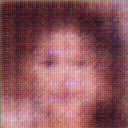
\includegraphics[width=150px]{500_fake_images/samples_5_404.png}%
\caption{A Man In A Black Shirt And A Tie}%
\end{figure}

%
\end{document}